%% General definitions
\documentclass{article} %% Determines the general format.
\usepackage{a4wide} %% paper size: A4.
\usepackage[utf8]{inputenc} %% This file is written in UTF-8.
%% Some editors on Windows cannot save files in UTF-8.
%% If there is a problem with special characters not showing up
%% correctly, try switching "utf8" to "latin1" (ISO 8859-1).
\usepackage[T1]{fontenc} %% Format of the resulting PDF file.
\usepackage{fancyhdr} %% Package to create a header on each page.
\usepackage{lastpage} %% Used for "Page X of Y" in the header.
                      %% For this to work, you have to call pdflatex twice.
\usepackage{enumerate} %% Used to change the style of enumerations (see below).

\usepackage{amssymb} %% Definitions for math symbols.
\usepackage{amsmath} %% Definitions for math symbols.

\usepackage{tikz}  %% Pagacke to create graphics (graphs, automata, etc.)
\usetikzlibrary{shapes,arrows,calc,positioning}
\usetikzlibrary{graphs}
\usetikzlibrary{automata} %% Tikz library to draw automata
\usetikzlibrary{arrows}   %% Tikz library for nicer arrow heads
\usetikzlibrary{positioning}    %% Tikz library for more positioning options

\usepackage{hyperref} %% hyperlinks

\usepackage{chessfss} % contained in debian package texlive-games

\usepackage{listings}   % include & display python code
\usepackage[edges]{forest}  % for search trees

\tikzset{WhiteSquare/.style = {shape=rectangle, minimum width=28, minimum
    height=28, anchor=south west}}
\tikzset{BlackSquare/.style = {shape=rectangle, fill=lightgray, minimum
    width=28, minimum height=28, anchor=south west}}

%% Left side of header
\lhead{\course\\\semester\\Exercise \homeworkNumber}
%% Right side of header
\rhead{\authorname\\Page \thepage\ of \pageref{LastPage}}
%% Height of header
\usepackage[headheight=36pt]{geometry}
%% Page style that uses the header
\pagestyle{fancy}

\newcommand{\authorname}{Benjamin Regez\\Luis Tritschler}
\newcommand{\semester}{Spring Semester 2026}
\newcommand{\course}{Foundations of Artificial Intelligence}
\newcommand{\homeworkNumber}{10}

\renewcommand{\thesection}{Exercise \homeworkNumber.\arabic{section}}


\begin{document}

\section{}
\begin{enumerate}[(a)]
    \item $h^*(I) = 3$
    \item $h^+(I) = 3$
    \item RPG for $\Pi$:\\[1em]
    \begin{center}
    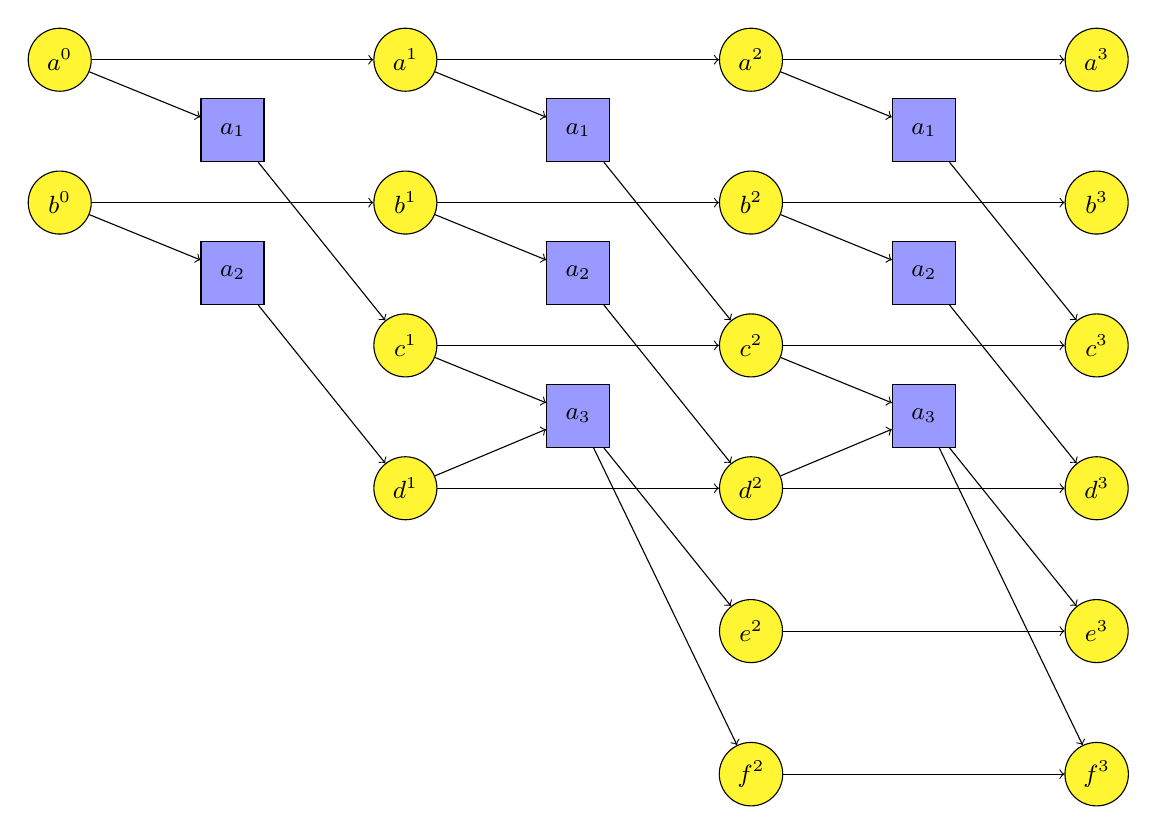
\begin{tikzpicture}[
    node distance=1cm and 1.5cm,
    every node/.style={font=\small},
    state/.style={circle, draw, fill=yellow!80, minimum size=8mm},
    action/.style={rectangle, draw, fill=blue!40, minimum size=8mm},
    goal/.style={rectangle, draw, fill=red!80, minimum size=10mm}
    ]
    % Layer 0
    \node[state] (a0) {$a^0$};
    \node[state, below=of a0] (b0) {$b^0$};
    % Actions between 0 and 1
    \node[action, below right=0.2cm and 1.5cm of a0] (a11) {$a_1$};
    \draw[->] (a0) -- (a11);
    \node[action, below right=0.2cm and 1.5cm of b0] (a12) {$a_2$};
    \draw[->] (b0) -- (a12);
    % Layer 1
    \node[state, above right=0.2cm and 1.5 of a11] (a1) {$a^1$};
    \draw[->] (a0) -- (a1);
    \node[state, above right=0.2cm and 1.5 of a12] (b1) {$b^1$};
    \draw[->] (b0) -- (b1);
    \node[state, below=of b1] (c1) {$c^1$};
    \draw[->] (a11) -- (c1);
    \node[state, below=of c1] (d1) {$d^1$};
    \draw[->] (a12) -- (d1);
    % Actions between 1 and 2
    \node[action, below right=0.2cm and 1.5cm of a1] (a21) {$a_1$};
    \draw[->] (a1) -- (a21);
    \node[action, below right=0.2cm and 1.5cm of b1] (a22) {$a_2$};
    \draw[->] (b1) -- (a22);
    \node[action, below right=0.2cm and 1.5cm of c1] (a23) {$a_3$};
    \draw[->] (c1) -- (a23);
    \draw[->] (d1) -- (a23);
    % Layer 2
    \node[state, above right=0.2cm and 1.5 of a21] (a2) {$a^2$};
    \draw[->] (a1) -- (a2);
    \node[state, above right=0.2cm and 1.5 of a22] (b2) {$b^2$};
    \draw[->] (b1) -- (b2);
    \node[state, below=of b2] (c2) {$c^2$};
    \draw[->] (a21) -- (c2);
    \draw[->] (c1) -- (c2);
    \node[state, below=of c2] (d2) {$d^2$};
    \draw[->] (a22) -- (d2);
    \draw[->] (d1) -- (d2);
    \node[state, below=of d2] (e2) {$e^2$};
    \draw[->] (a23) -- (e2);
    \node[state, below=of e2] (f2) {$f^2$};
    \draw[->] (a23) -- (f2);
    % Actions between 2 and 3
    \node[action, below right=0.2cm and 1.5cm of a2] (a31) {$a_1$};
    \draw[->] (a2) -- (a31);
    \node[action, below right=0.2cm and 1.5cm of b2] (a32) {$a_2$};
    \draw[->] (b2) -- (a32);
    \node[action, below right=0.2cm and 1.5cm of c2] (a33) {$a_3$};
    \draw[->] (c2) -- (a33);
    \draw[->] (d2) -- (a33);
    % Layer 3 = n
    \node[state, above right=0.2cm and 1.5 of a31] (a3) {$a^3$};
    \draw[->] (a2) -- (a3);
    \node[state, above right=0.2cm and 1.5 of a32] (b3) {$b^3$};
    \draw[->] (b2) -- (b3);
    \node[state, below=of b3] (c3) {$c^3$};
    \draw[->] (a31) -- (c3);
    \draw[->] (c2) -- (c3);
    \node[state, below=of c3] (d3) {$d^3$};
    \draw[->] (a32) -- (d3);
    \draw[->] (d2) -- (d3);
    \node[state, below=of d3] (e3) {$e^3$};
    \draw[->] (a33) -- (e3);
    \draw[->] (e2) -- (e3);
    \node[state, below=of e3] (f3) {$f^3$};
    \draw[->] (a33) -- (f3);
    \draw[->] (f2) -- (f3);
    \end{tikzpicture}
    \end{center}
    \item TODO
    \item TODO
    \item TODO
\end{enumerate}

\section*{Statement on scientific integrity}
\begin{itemize}
    \item For 10.1(c) we asked ChatGPT for help with the \texttt{tikzpicture} library
\end{itemize}
Content-wise, we solved the entire exercise sheet on our own.

\end{document}
